\section{Governance}
Tagion is a common resource(s) that constitutes the network, Tagion trademark, code and governance mechanisms, which are governed by a common resource governance model. The model is based on the ideas and design principles of Elinor Ostrom's work with the (self-) governing of the commons. The overall perception of resource governance in today's society is between the extremes of private or state ownership. There is a third option called Commons, which can be translated to self-governance or community governance. It is much more efficient as well when it comes to the governing of common resources, as Elinor Ostrom argues and proves. She won the Nobel Prize in Economics in 2009 for her work within the field \cite{ELINOR_OSTROM_NOBEL_LECTURE, 10.1257/aer.100.3.641}. We believe a monetary system and banking network should be a common resource because all users of it have an equal interest in the system; thus, the system should serve all interests equally by being governed as a common resource. Designing a governance model for a common requires clear rules for the boundaries, resources and actors in the system, which is described in this chapter. \cite{10.2139/ssrn.997834, ALLEN_CHRISTOPHER, ostrom2006}
\newline
Tagion has three main governance types that are listed in \cref{tab:governance_types} and elaborated in the next sub-sections. The common resources of Tagion are elaborated in \cref{sec:common_resources}.

\begin{table}[H]
 \begin{center}
  \begin{tabular}{|p{3cm}|p{8.5cm}|}
   \hline
   Governance Type & Purpose \\
   \hline
   Node & Defines rules and processes for nodes.\newline
   I.e. algorithms controlling the node scoring model and proof-of-people protocol. \\
   \hline
   Economic & Defines rules and processes for ecnomics in the system. \newline
   I.e. algorithms controlling the rewards and fees. \\
   \hline
   System Upgrade & Defines rules and processes for system upgrades. \newline
   I.e. algorithms for node software upgrades and script function upgrades.\\
   \hline
  \end{tabular}
 \end{center}
 \caption{Overview of the three main governance types for the system: Node, Economic and System Upgrade Governance.}
 \label{tab:governance_types}
\end{table}


\subsection{Node Governance} \label{sec:node_governance}
The purpose of Node Governance is to ensure a stable network and that all nodes agrees on the state of the network. The Node Governance is devided into layers of governance as it is defined in \cref{tab:node_governance_layers} and the Node Governance only governances procedures which can be automatomated via algorithms. This section does not inlcude the rules for the user of the network, only the rules for automated nodes. 
\begin{table}[H]
 \begin{center}
  \begin{tabular}{|p{4cm}|p{8cm}|}
   \hline
   Node Layers & Governance Rules \\
   \hline
   Join Layer & Ruling the selection of nodes to join the network. \\
   \hline
   Prospect Layer &  This layer governance the rules to be selected as an node validator. \\
   \hline
   Available Layer & Governance for the validators. \\
   \hline
   Active Layer & Governance the rules of the validators which performs the actual validation work.  \\
   \hline  
  \end{tabular}
 \end{center}
 \caption{The actors in the Tagion Network.}
 \label{tab:node_governance_layers}
\end{table}


A node is defined as an automatomated-unit (computer) which can send/receive information to any other node in a network. The nodes are devided up into node-actors as defined in \cref{tab:node_actors}.
\begin{table}[H]
 \begin{center}
  \begin{tabular}{|p{4cm}|p{8cm}|}
   \hline
   Node Actor & Description \\
   \hline
   External Node \bfit{XN} & Nodes not available for the network.\\
   \hline
   Prospect Node \bfit{PN} & Nodes waiting to become a \bfit{N}. \\
   \hline
   Available Node \bfit{N} & Nodes avliable to be select as a \bfit{RN}. \\
   \hline
   Reserve Node \bfit{RN} & \bfit{PN} are a subset of \bfit{RN}, which are waiting to become a \bfit{AN}. \\
   \hline
   Active Node \bfit{AN} & \bfit{AN} are a subset of \bfit{N}. \bfit{AN} operate and constitute the live Tagion network. \\
   \hline  
  \end{tabular}
 \end{center}
 \caption{The Node actors in the Tagion Network.}
 \label{tab:node_actors}
\end{table}


\begin{figure}[H]
 \centering
 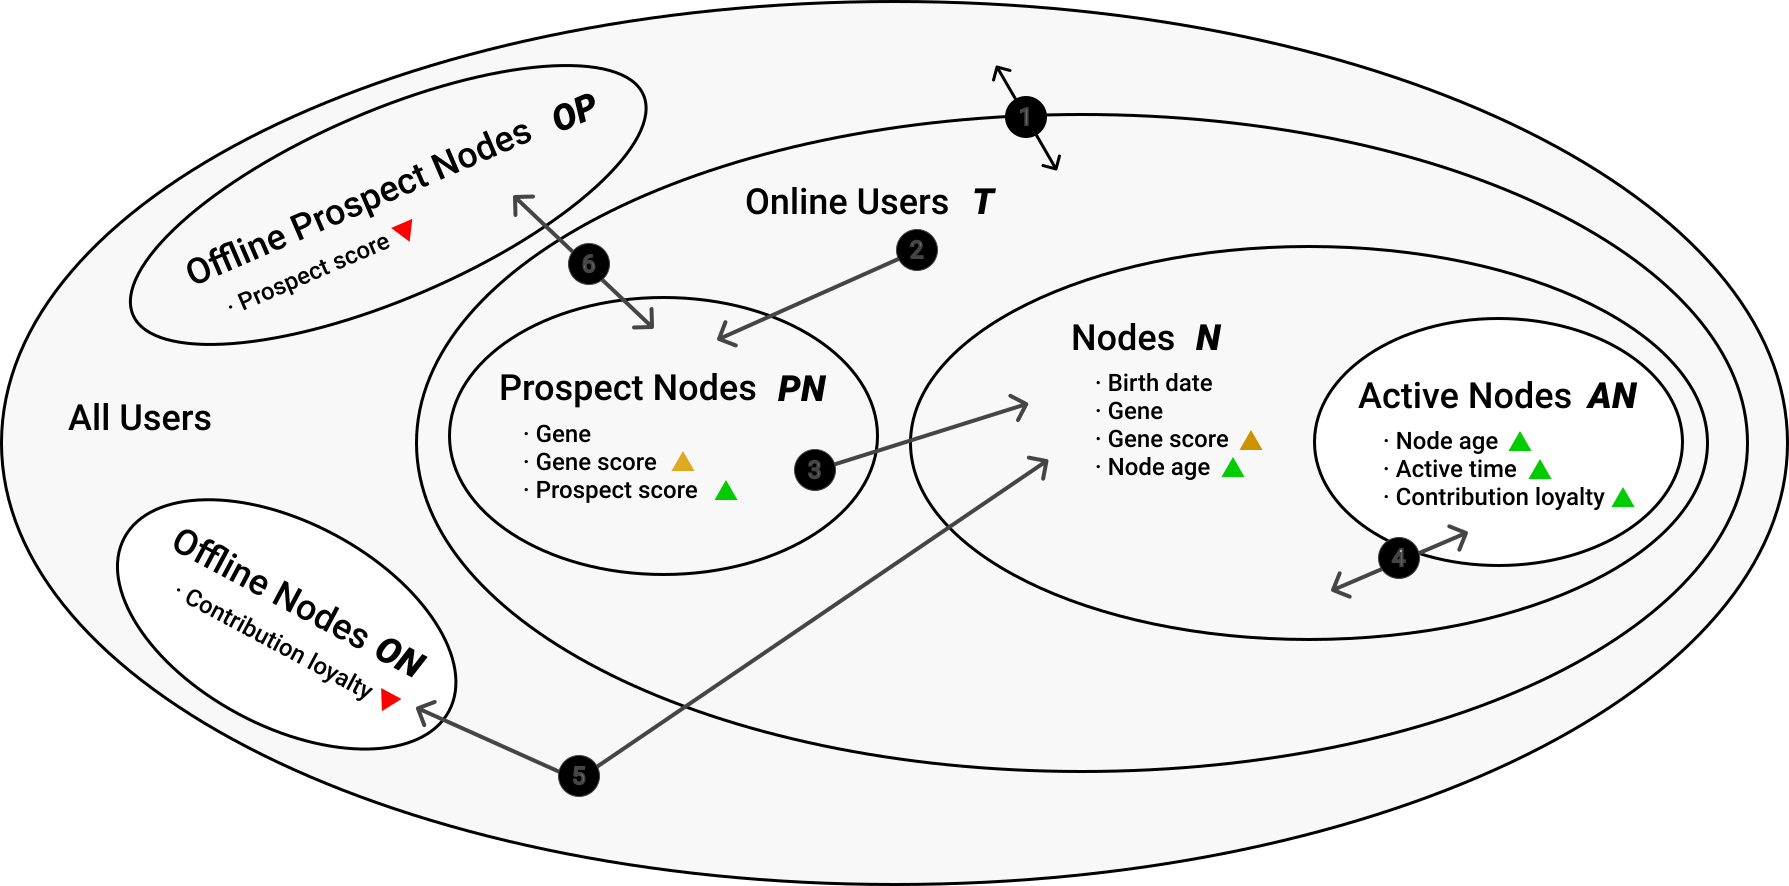
\includegraphics[width=1.05\textwidth]{fig/governance_model.pdf}
 \caption{Governance Model with actors, boundaries and variables in the Tagion system. The green triangle indicates an increase for the actor, the red triangle a decrease and the yellow an increase after an action i.e. a mating transaction.}
 \label{fig:governance_model}
\end{figure}


The boundaries are labelled with numbers in \cref{fig:governance_model} which are defined as:
\begin{enumerate}
 \item Any node can go from online to offline and vice versa. The network is open for all; it means that anyone who has not yet used the system can become a user as well. 
 
 \item Any node can become a validator-node over time and must first become a prospect node. The transition is based on a random selection, a lottery, to help ensure a broad representation of nodes. When going from a user to a prospect node or node, in general, the user is no longer anonymous, but a public servant with a public name record in the system \cref{sec:name_card_contract}.
 
 \item When a prospect nodes have been socially verified and earned enough prospect score that is being available for the network for a period of time then the prospect node becomes a node, i.e. born and receives a gene number and a birth date.
 
 \item Nodes are chosen randomly within a given interval continues to be active nodes, and active nodes are chosen randomly to be inactive nodes. Nodes and active nodes are swapped back and forth continuously to make it impossible to predict, which nodes are active in 10 minute intervals, enhancing security. A node is selected by a \abbrev{UDR}{Unpredictable Deterministic Random} algorithm, where the probability of being chosen as an active node or to continue as an active node depends on four variables:  \abbrev{gs}{Gene score},  \abbrev{at}{active time},  \abbrev{no}{node age} and \abbrev{cl}{contribution loyalty}. 
 \begin{equation}
  P_{(active)} (gs, cl, na/at)
 \end{equation}
 
 \item A node can go from online to offline and vice versa, if offline, it is not possible to be an active node or to become an active node. 
 
 \item A prospect node can go from online to offline and vice versa. 
\end{enumerate}

\subsubsection{External Node Layer} \label{sec:extenal_node_layer}
xxx

\subsubsection{Prospect Node Layer} \label{sec:prostect_node_layer}
xxx

\subsubsection{Available Node Layer} \label{sec:available_node_layer}
xxx

\subsubsection{Active Node Layer} \label{sec:active_node_layer}
xxx


\subsubsection{Reputational Scoring Model} \label{sec:reputational_scoring_model}
The model consists of actors, variables and the boundaries of the actors, including the transition over a boundary.


The variables of the actors and scoring rules for the model are defined in \cref{tab:governance_variables}.
\begin{table}[H]
 \begin{center}
  \begin{tabular}{|p{4cm}|p{8cm}|}
  \hline
  Variable name & Definition and scoring rule \\
  \hline
  Birthdate & The date a prospect node becomes a node. \\
  \hline
  Gene & A gene is unique for each node. \\
  \hline
  Gene score (Gene-diversification points) & Each time a node mates with another node, a score is calculated for them both based on how diverse their genes are compared to each other. They mate each time verification of a prospect node takes place, when an active node makes an epoch, see \cref{sec:hashgraph_cm}, and when two nodes choose to mate and validate each other. \\
  \hline
  Node age & A measure of a node's total available time for the network. Time as both a node and an active node. It increases both as a node and active node when available for the network. \\
  \hline
  Active time & Time as an active node. It increases when a node is active.\\
  \hline
  Prospect score & The Prospect score variable is a measure of how much the prospect node has been available to the network. It increases when the prospect node is available and decreases when not. \\
  \hline
  Contribution loyalty & A measure of how much the node has been active and stayed available. Non-availability of a node decreases contribution loyalty; being an active node increases loyalty. \\
  \hline
  \end{tabular}
 \end{center}
 \caption{Variables and scoring rules for the reputational scoring model}
 \label{tab:governance_variables}
\end{table}


The actors with their boundaries to each other and variables are illustrated in \cref{fig:governance_model}, the boundaries and transition over them are described below.



\subsubsection{Proof-of-People} \label{sec:proof-of-people}
The Proof-of-People protocol is a heuristic protocol with a random and social component. Heuristic, because it aims to secure the democratic principles of one person one node and that it is an actual person behind a node. One person one node cannot be accomplished, but the social component would accomplish an approximation to this. The social component makes it difficult to manage more than one node, and the scoring mechanism makes it less favourable. The approximation would ensure a highly-distributed system when it is combined with a random selection of new prospect nodes. It means no actor or a few actors would control the network when the number of nodes has a certain size, making it secure.

The protocol for becoming a node is:

\begin{enumerate}
 \item A user creates or has a name record in the system, see \cref{sec:name_card_contract}. 
 
 \item A user has a name record with an age of more than one month. The user makes a prospect node record transaction where a node-transaction fee is paid together with a staked amount. The prospect node record contains the user's public key, has the stake attached to it and is linked to the name record.
 
 \item With an average of 10 minutes, a prospect node record is chosen randomly, which burns the stake and gives a node coupon. Then the prospect node should send a proof of activity from within seven days. The proof is simply a public key to a bill in the DART, which are created within the last seven days. 
 
 \item When the user has sent the proof, two random active nodes verify the proof and give a gene to the prospect by crossing their genes with each other. The gene is added to the prospect node record and both parents sign the prospect node record. 
 
 \item \label{itm:mating_transaction} The rewarded node in the same epoch as where the coupon was issued is the first to identify the prospect in a dialogue. If the rewarded node validates the prospect, they make a mating transaction, which both signs. Both nodes receive gene score points for this transaction, and the mating transaction is linked to the prospect node's record. The gene score points are symbolised with the yellow triangle on \cref{fig:governance_model}. 
 
 \item Two semi-determined identifications should be made by two of the next ten epoch rewarded nodes. The prospect engages in a dialogue with potential validators to get two mating transactions. This is the same mating transaction as in \cref{itm:mating_transaction}.
 
 \item Now the node has received three identifications, which means it can start participating as a prospect node on the network, and receive prospect score points. When the node has reached a prospect score threshold the step is completed. 
 
 \item A second semi-determined identification of the prospect is made with two nodes from the last ten epochs from the point the prospect score is reached. This is the same mating transaction as in \cref{itm:mating_transaction}. 
 
 \item The last mating transaction creates a birth date in the prospect node record, making the prospect node a full node on the network. 
\end{enumerate}

There are three main components to the protocol:
\begin{enumerate}
 \item The first selection of prospect nodes introduces a certain time-lag by the need to have a name record with an age of one month and a stake amount. A node transaction fee ensures that small and zero transactions cannot be used to increase the chances of winning the coupon. The fee and stake ensure commitment as well.  
 \item The requirement of activity within the last seven days creates a requirement for the user to have activity in the network. 
 \item A social component that forces new nodes to engage in dialogue with other nodes, thus creating relations and communities. It is a local or virtual identification and dialogue with each other following the protocol. Both parties receive gene score points when mating, thus raising the chance for rewards to create a direct economic incentive and, indirectly, by ensuring non-evil nodes in the system, ensure the long-term sustainability and economic network worth of the system. Therefore, all nodes have a natural incentive to ensure that new nodes are real persons with honest intentions.
\end{enumerate}

A premise for the social protocol to work is that users engage in dialogue; it requires social responsibility and engagement. As long as this premise is true, the node governance components can be adjusted based on the real experience with the test network, where a balance between the work and drag of being and becoming a node compared to actual user adoption and distribution. \newline
Besides the proof-of-people protocol, a continuous evaluation of nodes can be imaged. E.g. each month, all nodes need to engage in dialogue with 3 other nodes receiving gene score points. 
More, the future perspectives of the sharding of the network would allow the network to be more local based, thus removing cultural and language barriers, which can foster people to educate each other and build a culture around the network. 

That is accomplished by a reputational scoring model and a proof-of-people protocol that is a social heuristic protocol. Both components are inspired by Charles Darwin's evolutionary theory of how species best survive in a new environment with the two main elements 1) most diversified paired genes and 2) caretaking of the offspring. These two elements are embedded in the scoring model and protocol. 

\paragraph{Defining a node} is done from democratic principles, where all can participate and where one person has one vote. These principles are translated into a permissionless system where one node has one vote, and where one person only controls one node. It would ensure full distribution of nodes because centralisation is not possible. It is not possible to ensure 100\% that one person can only control one node, but it is the aim. More, it is not required that the network is fully distributed to ensure the network is secure. The requirement is that it is distributed in a way, where many actors control an insignificant amount of nodes, thus avoiding the centralisation of power like in other networks, where few nodes may have majority control. \\
One of the downsides of democracy is that all have the same voting power independent of contribution. Thus, the Tagion system has a scoring system that values loyalty, that is, work through time, but still is open and fair for all to participate. The social component in the proof-of-people protocol tries to ensure that one person only has one node and is a real person. The protocol also selects users randomly to become nodes ensuring even distribution and fairness.  


\subsection{Economic Governance} \label{subsec:economic_governance}
The economic model of Tagion tries to stabilise the intrinsic value of the system, rather than being pegged to external currencies or assets. 
There are two main phases of economic governance, where the first is a linear and stable supply. The second phase builds on a model that aims to keep the intrinsic value of the currency stable by controlling the supply of money. 

The idea is that money reflects the underlying value of an asset; money in itself does not have value. Production in our society creates the value: the assets, which values are represented by money, make them easy to trade. Being able to represent a value for the persons using the money includes the need to trust that they can use the money elsewhere, and it needs to have a stable value over time. 
The reason a currency is trusted is that it has adoption and a stable value over time, and not because money is backed by gold or is state-backed. Adoption of the Tagion network happens over time, but the stability of the Tagion currency needs to be addressed, making it trusted. 


\subsubsection{Stable supply}
Creating a stable supply with full transparency like in Bitcoin (though decreasing supply, stable) creates trust in the system. No actor can create a significant supply and dilute the value and the trust in the system. 
Some systems have a built-in cap in the system, which needs to be changed programmatically, like Bitcoin. Tagion does not have a built-in cap, because the supply of money should somehow correspond to the adoption, and thus the representation of values in the system. Otherwise, destructive deflation in the system could cause the real use of the system to fall, because people would then tend to hold and speculate with the money instead of using it. Of course, inflation can also be destructive, but a steady and insignificant increase in the supply of money should not create hyperinflation in the system. The most important thing would be that people keep using Tagions because they trust the money and do not hold on to them due to deflation.
During the first couple of years in a monetary system's lifetime, high volatility is expected because of the low numbers of actors, which can easily both make the internal and external value go up and down because each actor's transaction can be significant in the system. As adoption occurs and the number of actors in the system becomes significant compared to a single actor, then price volatility decreases, because no single actor has a significant effect on the system. When this adoption size is reached, it leads us to the next phase, where an algorithm controlling the money supply stabilises the intrinsic value. 

\subsubsection{Stable intrinsic value}
Milton Friedman stated that ``Inflation is always and everywhere a monetary phenomenon''. This means that inflation has nothing to do with the production in society \cite{friedman_counter}. The relationship between money and the production in society can be expressed by the equation of exchange: \cite{britannica_monetarism}

\begin{equation}
 M \cdot V = P \cdot Q
 \label{eq:equation_of_exchange}
\end{equation}

\begin{itemize}
 \item[$M$]is the quantity of money. 
 \item[$V$]is the velocity of money (the number of times per year the average currency in the money supply is spent).
 \item[$P$]is the average price level of sold goods and services.
 \item[$Q$](or Y) is the real GDP for an economy.
\end{itemize}

This equation has some useful constructs of the measure of money within a monetary system, but also an external measure of GDP, which is not available for Tagion because Tagion only measures on internal variables. Tagion sees an economic system as a flow system and not as static equilibrium. The constructs in the model are used but translated into a dynamic flow model with only internal variables. A translation of the constructs to variables in the Tagion system could be: 

\begin{itemize}
 \item[$M$]is the quantity of Tagions in the system. That is a variable directly measurable in the system.  
 \item[$V$]is the number of times per year the average Tagion in the money supply is spent. It can be mapped to the variable of the number of transactions and average supply of money per year, which are direct variables in the system. 
 \item[$Q$]can be mapped with an average number of nodes in the system, which is an expression for users, and adoption in the system, thus how much of users' value the system represents. More variables, such as the acceleration of transactions, average transactions per time unit, average transaction size and acceleration can all be potential variables for the constructs in the system.
 \item[$P$]is the average price level in the Tagion monetary system, which can be expressed as: 
 \begin{equation}
  P = \frac{M \cdot V}{Q}
 \end{equation}
 The aim would be to keep the price level $P$ stable, where the only controlled variable is the supply of money, which can be regulated after a model by an algorithm. 
\end{itemize}

These variables need to be modelled, and construct-validation, correlation and causal-relation tests made. It requires a system of a particular size and much testing to model this. Tagion is confident that it is possible to keep intrinsic stability by such a model in the system. 
The aim is not an xx \% inflation target of the system, which makes no sense when external constructs as GDP are not measured, but to keep the intrinsic value in the system stable. It is accomplished by creating the adoption of the system and an intrinsic stability mechanism in the system. It should generate long-term trust and stability over time, becoming a store of value. External parties must not control the money supply and system with their interest which dilutes the trust and value of the money. 

\subsection{System Upgrade Governance}
Upgradability has been taken into consideration on two main levels: Node Software, which concerns the actual base protocols for running a node, and Script Function Upgrades, which concerns the function scripts in the network. All scripts are stored in the DART, meaning it does not require an upgrade of the base protocols, but just a change of the script function state in the DART. Function scripts are node governance and economic governance algorithms.

\subsubsection{Node Base Protocol Upgrade}
The upgrade of the node base protocols should be backwards compatible with the previous version. It means the software can run the current network version and the new one, but it does not mean the networks are compatible, which can be divided into two categories minor and core upgrades:

\paragraph{Minor and bug-fixes upgrades}
This upgrade does not change the structure of the database and core algorithms, meaning that it can run in the same network as the current. It requires 5/6 of the active nodes to approve the upgrade. 
\paragraph{Core and structural upgrades}
Core and structural upgrades make hard changes, which can be core algorithms for cryptography or the structure of the database, which make the current network incompatible with the new one. It means that the nodes approving the new network operate both the current and new network in parallel until the upgrade is approved. It requires a 5/6 majority of the active nodes to approve the upgrade and to enforce the new network version. 
\paragraph{Script Function Upgrades}
Script function upgrades are when a script in the database in the network is changed, created or deleted. It does not require the installation of a new binary on the computer the node is running on. Before a new function is approved, 5/6 of the active nodes need to approve it.

\subsection{Common Resources} \label{sec:common_resources}
The Tagion network is a common resource, meaning that no state or private entity should own it because it serves a common purpose for the whole community and the users of the system. 

The resources are the actual network, and the governance mechanism all the IP (intellectual property) related to Tagion, which is listed below.

\subsubsection{Open Source code}
The source code is released under a GNU GPL or similar license and owned by the Tagion Foundation. The licensing is in process. Closed or commercial projects do need permission to use the source code.
At the moment the git repository is not opened. Preparations to open the repository are being made.
Before the open-source license is defined, and the open patent license has been given to the Tagion Foundation from I25S ApS, the repository cannot be opened. It is planned to open the project as soon as possible. People with legitimate reasons to verify the code can write to info@tagion.org and a copy of the source code can be shared after a signed NDA is in place.

\subsubsection{Patents}
EU patents are filed in the company name I25S ApS. The patents concern 1) a database system and 2) a network gossip protocol.
The database system, which is implemented as the DART in Tagion, is a distributed database system that can efficiently search and store data based on a cryptographic hash enabling the network to execute transactions in parallel thus promoting performance and scalability.
The gossip protocol is an efficient way to share information among all members of the network.

\paragraph{Open Licenses}
An open license is defined to be a free patent license given to the open-source project that cannot be revoked.
All open-source projects having the same type of license as the Tagion Project are as a rule of thumb granted a free license that cannot be revoked automatically.
Other open-source projects need to apply for an open license. The licenses cannot be revoked when first given.
The Tagion Foundation and project is given an open license by I25S. Projects that fork the Tagion code need an open license by default.

\subsubsection{“Tagion” Trademark}
An EU Trademark is registered for “Tagion” and owned by the Tagion Foundation including related internet domains. 
The reason for the trademark is to make sure that projects, which are forking the source and governance model, cannot call themselves Tagion XYC. It confuses the end-users and community, thus multiple projects with similar names should be avoided.
Tagion can protect itself from other projects or entities that wish to associate themselves with Tagion for malicious purposes.


